\chapter{Síntesis de imágenes de radiointerferometría}
\label{cap:imagesynthesisinterferometry}

\section{Atacama Large Millimeter-Submillimeter Array}

El Atacama Large Millimeter-Submillimeter Array (ALMA) es un radiointerferómetro compuesto de 66 antenas de alta precisión que operan a un ancho rango de frecuencias milimétricas y submilimétricas. Cincuenta de estas antenas miden 12 metros de diámetro y son utilizadas para síntesis de imágenes de alta resolución. Por otra parte, esto es complementado por el \textit{Atacama Compact Array} también llamado \textit{Morita Array} compuesto por doce antenas de 7 metros de diámetro y por otras 4 antes de 12 metros diámetro para observaciones de poder total (\textit{Total Power}).

El conjunto de antenas está ubicado en el llano Chajnantor, un sitio que ofrece un cielo claro y un aire seco como condición requerida para observar en ondas milimétricas y submilimétricas.

La distribución de las antenas cede paso a lo que es llamado \textit{baseline} o distancia entre un par de antenas, que van desde 15 Km. hasta 16 Km. aproximadamente. Tanto la distribución de antes como la distancia entre éstas es crucial en la determinación de la calidad de la imagen y la resolución de ALMA \citep{alma-handbook}.

\begin{figure}[h!]
\centering
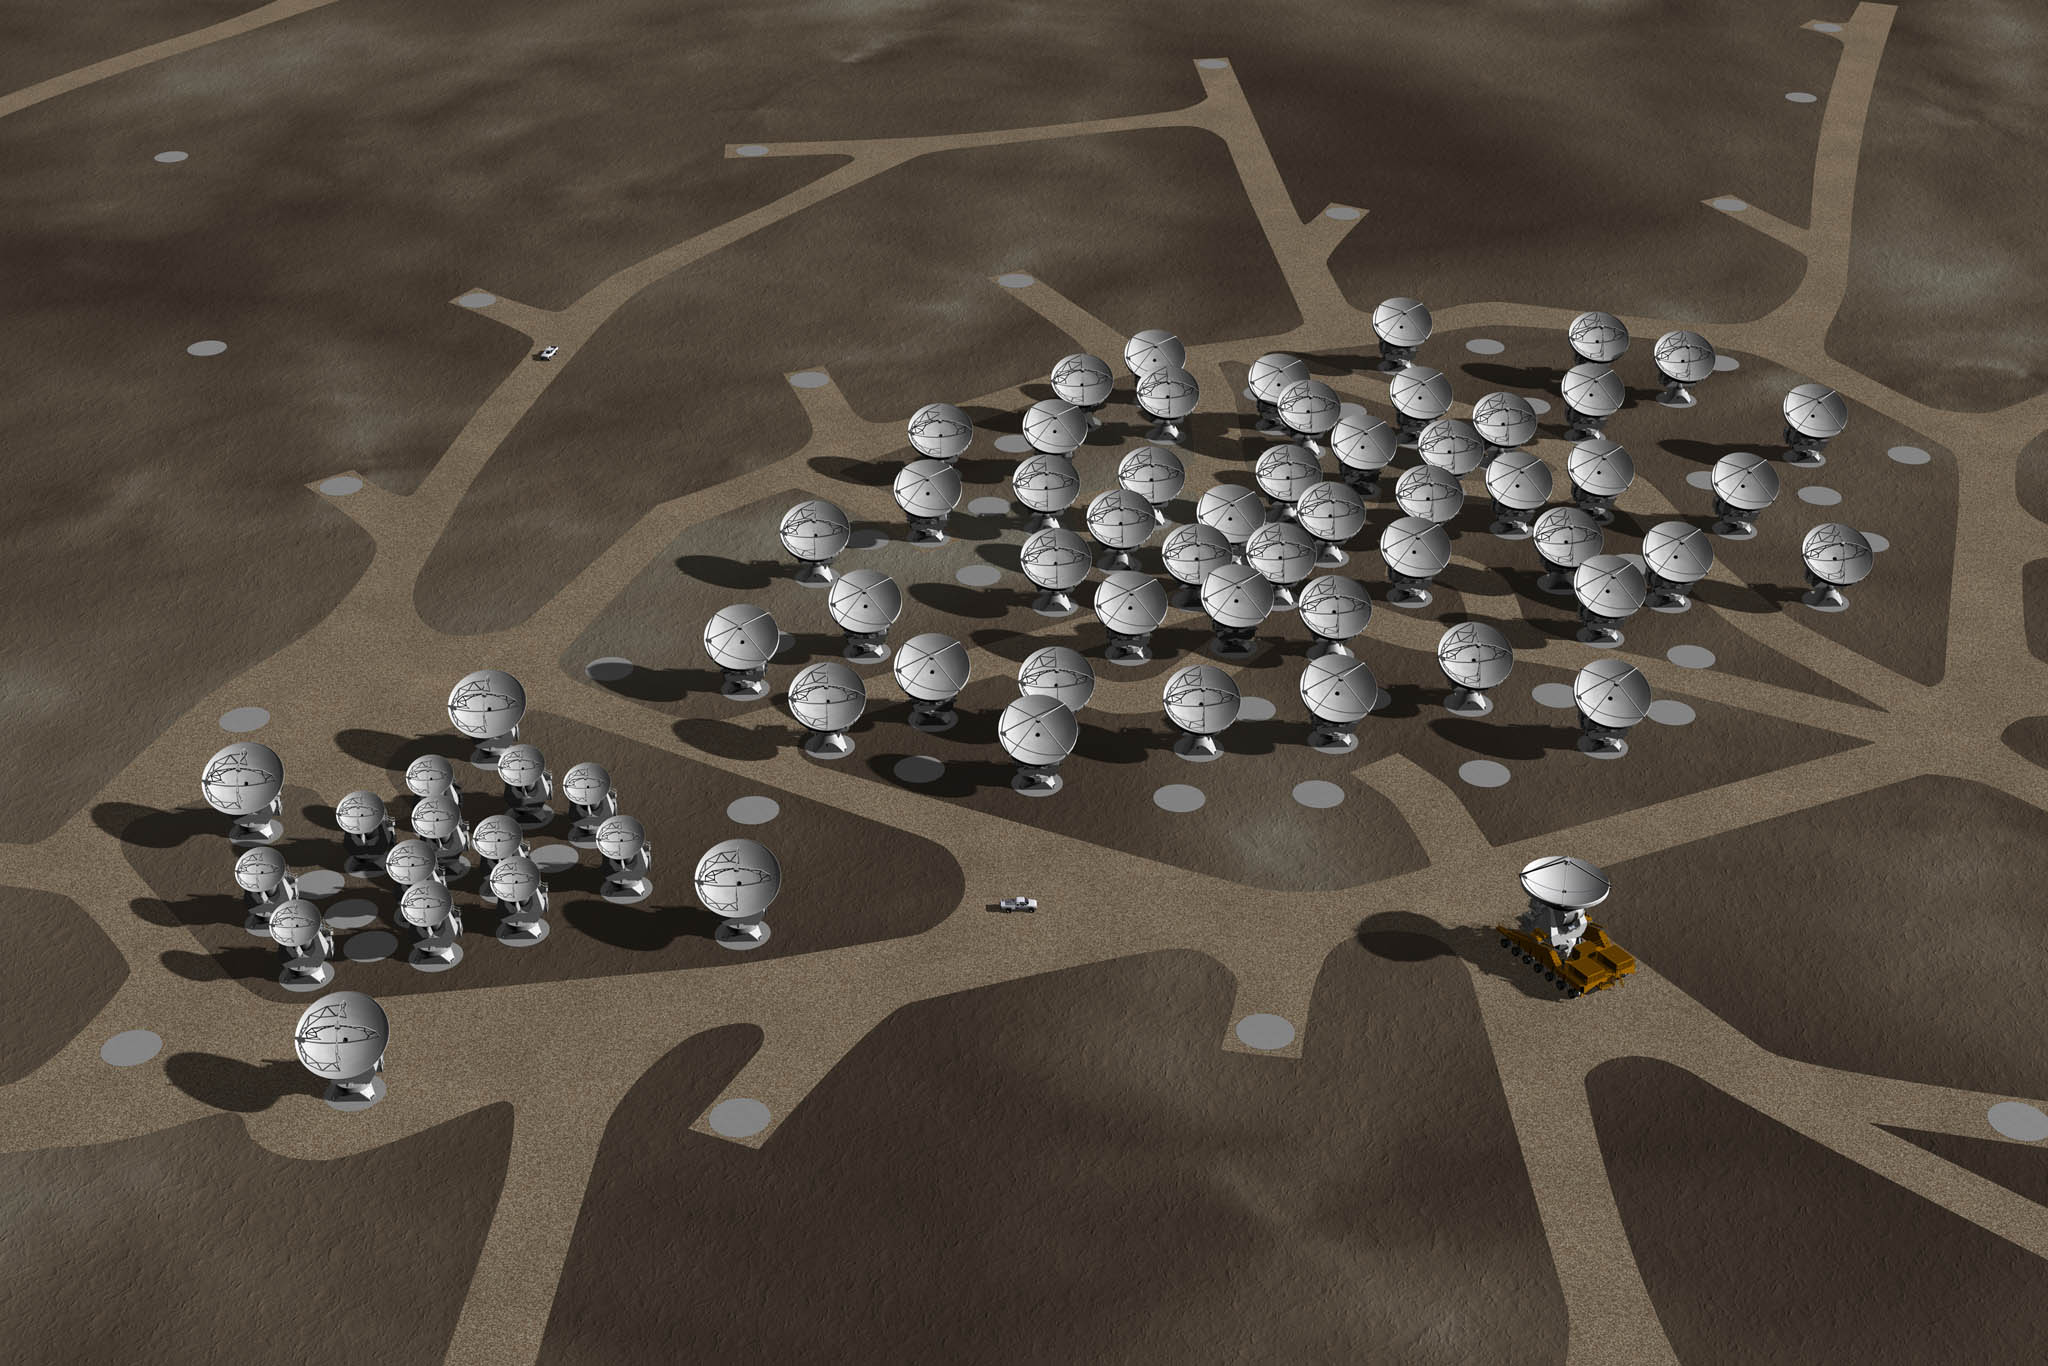
\includegraphics[scale=0.2]{images/almaarray.jpg}
\caption{Distribución de antenas en el llano Chajnantor. Fuente: ALMA (ESO/NAOJ/NRAO)}
\label{fig:almaarray}
\end{figure}

Por otro lado, cada antena contiene un receptor (también llamado \textit{Front-end}) que permite que las éstas capten información en diez bandas de frecuencia diferentes. Para ello cada antena está equipada con un criostato y su criorefrigerador adjunto. Estos criostatos contienen receptores que están montados y pueden ser reemplazados de forma fácil. En la tabla se adjuntan los datos de las distintas bandas de frecuencia que ALMA puede cubrir gracias a su front-end.

\newcommand{\ra}[1]{\renewcommand{\arraystretch}{#1}}
\begin{table}[h!]
\centering
\ra{1.2}
\caption{Las 10 Bandas de frecuencia de ALMA}
\label{tab:data}
\begin{tabular}{@{}rcrrcr@{}} 
\toprule
 \multicolumn{1}{c}{{\bf Banda}} & \phantom{a} & \multicolumn{2}{c}{{\bf Rango de frecuencia (GHz)}}  & \multicolumn{1}{c}{{\bf Temperatura (K)}} \\
 \midrule
 1   && 31 - 45 &&  26\\
 2   && 67 - 90 &&  47\\    
 3  && 84 - 116 &&  60\\
 4  && 125 - 163 &&  82\\
 5  && 162 - 211 &&  105\\
 6  && 211 - 275 &&  136\\
 7  && 275 - 373 &&  219\\
 8  && 385 - 500 &&  292\\
 9  && 602 - 720 &&  261\\
 10  && 787 - 950 &&  344\\
 \toprule
\end{tabular}
\end{table}











\chapter{GPGPU}
\label{cap:gpgpu}

\section{Arquitectura Unificada de Dispositivos de Cómputo}
\subsection{Arquitectura}
\subsection{Peer-to-Peer}
\subsection{Direccionamiento virtual unificado}
\subsection{GPUVMEM}

\chapter{Pruebas}
\label{cap:pruebas}

\chapter{Resultados}
\label{cap:resultados}